\section{Quantity 2: Ghost Margin}

\intuitbox{If two holes are both illuminated at once, each one's beam forms its own
image on the retina. When the eye is exactly in focus, both images land in
the same spot --- one hole, or fifty, makes no visual difference. When the
eye is myopic, each beam focuses slightly in front of the retina, and
because the beams enter the eye at different lateral positions, they now
land at slightly different spots. Two spots close together just look like
extra blur; two spots far enough apart look like literal double vision.
}
\subsection{The Formula}
\begin{equation}
\Delta r = \frac{s \cdot M}{P_0 - M}
\end{equation}
where $s$ is the center-to-center separation of the two holes, $M$ is
myopia in diopters, and $P_0\approx 60$D is the eye's total optical power.
Notice $\Delta r \to 0$ as $M\to 0$ --- a focused eye cannot produce two
separate images no matter how the holes are arranged, which is exactly the
sanity check that let this project reject an earlier, wrong version of this
formula.

The design is ghost-safe for a given pair if $\Delta r$ stays below the
eye's own resolution limit for that blur level.

\begin{figure}[h]
\centering
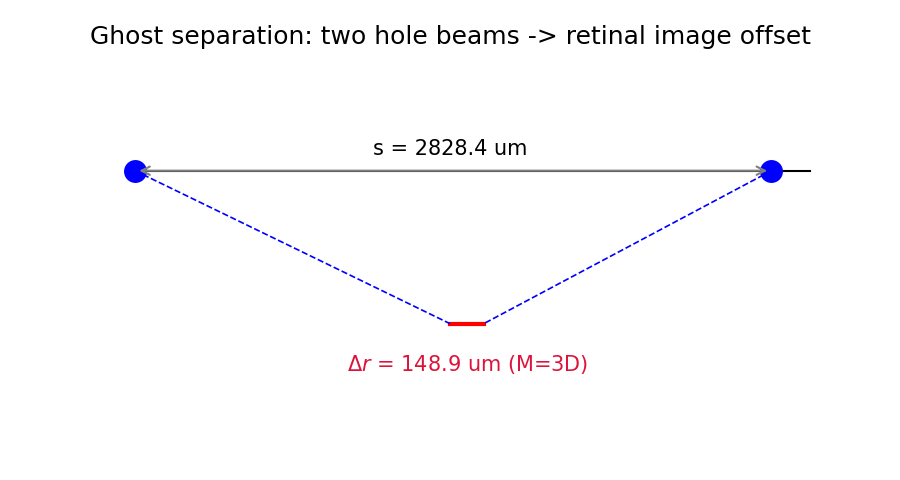
\includegraphics[width=0.75\textwidth]{verification_pdf_figs/fig_ghost.png}
\caption{Two holes separated by $s=2828.4\mu$m produce retinal images
separated by $\Delta r = 148.9\mu$m at $M=3$D, in the worked example of
Sec.~5.}
\end{figure}

\checkbox{Find the two closest illuminated holes in the design (usually the nearest
neighbors). Measure $s$ directly from their coordinates. Plug $s$, the
myopia level $M$, and $P_0=60$ into the formula above. Compare the result
against the resolvable-blur threshold reported for that $M$ --- if $\Delta
r$ exceeds it, that pair should have failed the safety check.
}
\newpage
